			
\section{Adversarial Search and Games}
	\subsection{Game}
		Un environnement multiagent peut etre vu comme un jeu et donc un problème résolut par recherche.
		Un jeux est défini par :
		\begin{itemize}
			\item \textbf{Initial state} : $S_0$ positions de debut du jeu
			\item \textbf{Player(s)} : quelle joueur a bougé
			\item \textbf{Actions(s)} : ensemble des mouvement légaux qu'il a fait
			\item \textbf{Result(s,a)} : modèle de transition qui définie le résultat du movement
			\item \textbf{Terminal set (s)} : test terminal du state
			\item \textbf{Utility(s,p)} :  valeur numérique du résultat du jeux pour le player $p$
		\end{itemize}
		
	\subsection{MinMax Algo}
	
		\begin{figure}[htp]
			\centering
			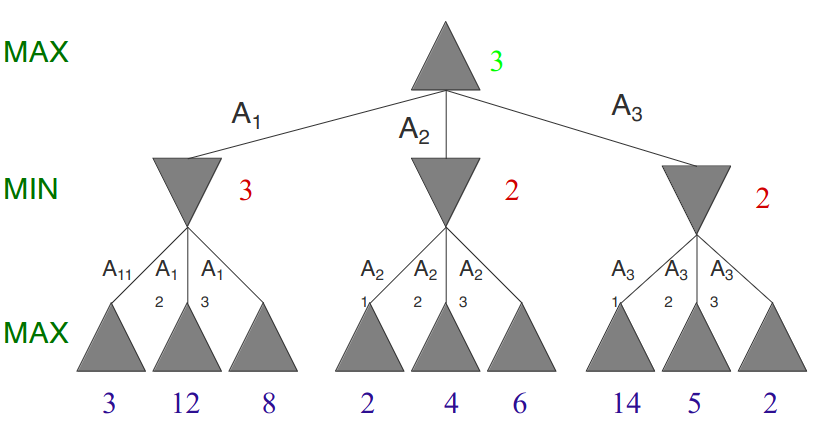
\includegraphics[width=0.7\textwidth]{img/minmax.png}
		\end{figure}
		
		Optimal pour les jeux déterministique et a 2 joueurs. 
		
		Chaque niveau représente a un jourer de jouer en fonction du state, un joueur (MAX) veut maximiser la valeur le deuxieme joueur (MIN) lui veut minimiser
		
		MinMax génère le tree entierement et applique une fonction d'utilité sur les derniers state (les leafs de l'arbre). Ensuite on remontre l'arbre en choissisant le MIN ou le MAX value en fonction du niveau de l'arbre (tours du joueurs). Le node final au dessus représente le meilleur mouvement possible

		\begin{figure}[htp]
			\centering
			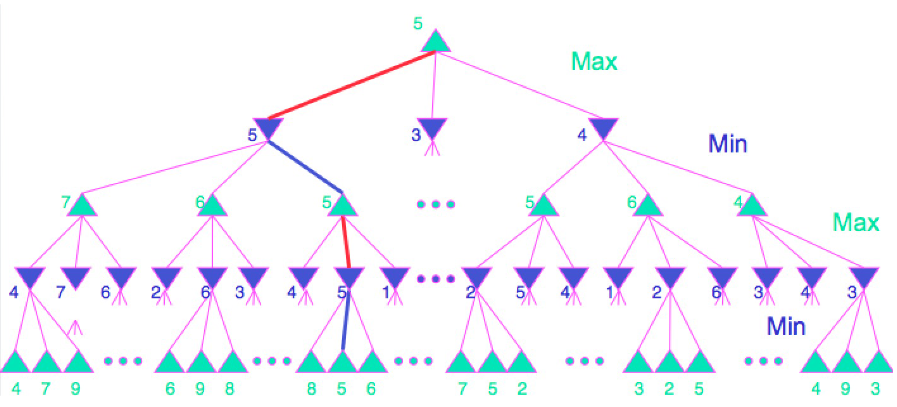
\includegraphics[width=0.7\textwidth]{img/exMinMax.png}
			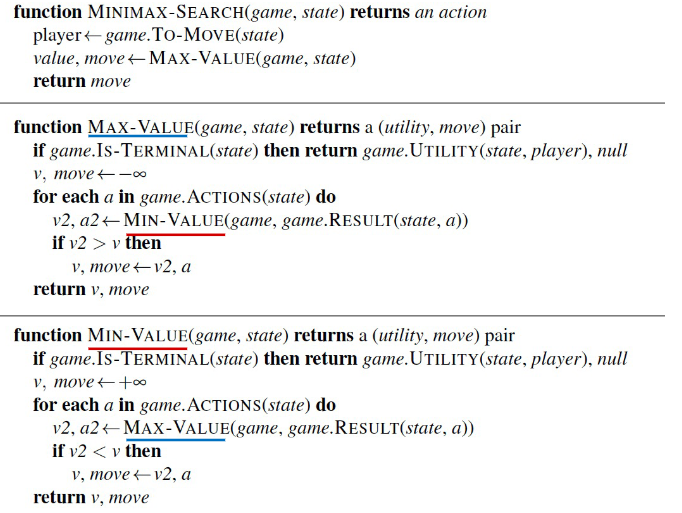
\includegraphics[width=0.7\textwidth]{img/algoMinMax.png}
		\end{figure}
		
		MinMax est basé sur DFS, est complet si le tree est finie. Il a une complexité de $\mathcal{O}(b^m)$ avec $b$ le facteur de branchement et m la profondeur max du tree.
		
		Il est possible de modifer l'algo pour avoir plus de 2 joueurs, il suffit de garder un vecteur a chaque node ou les élements du vecteur sont les utilité de chaque joueurs. Chaque joueur va choisir le mouvement qui maximise l'utilité
		
	\subsection{Alpha-Beta pruning}
		On cherche a "élagué" l'arbre afin de retirer les branche au quelle nous somme sur que il n'y a pas de meilleurs valeurs et donc inutile.Il n'affecte pas le resultat final
		\begin{figure}[htp]
			\centering
			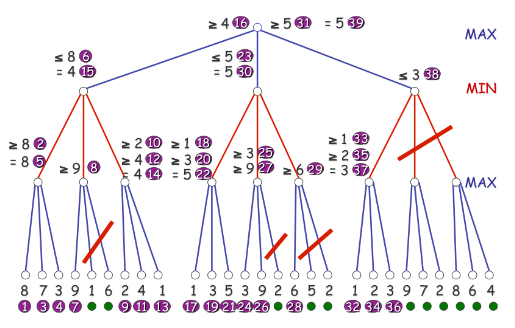
\includegraphics[width=0.7\textwidth]{img/alphabeta.png}
			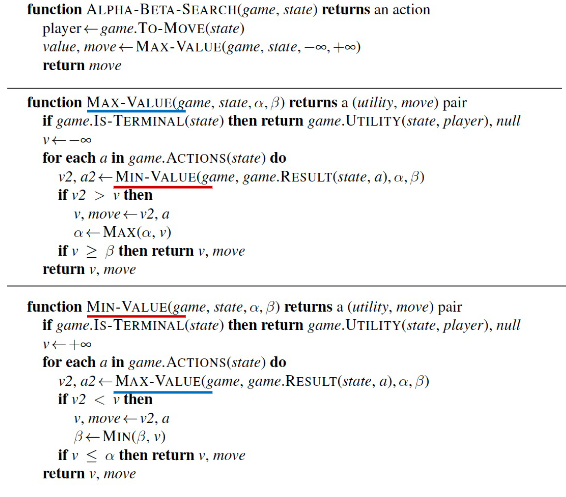
\includegraphics[width=0.7\textwidth]{img/alphabetaalgo.png}
		\end{figure}
		
		$\alpha$ : Valeur du meilleur (plus grande) choix trouvé d'ici la depuis les path visité pour MAX
		
		$\beta$ : Valeur du meilleur (plus petit) choix trouvé d'ici la depuis les path visité pour MIN
		
		Si les sucesseur de l'arbre sont idéalement visité, la complexité temporelle est alors de $\mathcal{O}(b^{d/2})$ et si visité random $\mathcal{O}(b^{3d/4})$
		
		
		\subsubsection{Move ordering}
	
			La disposition des nodes est idéal si le meilleur node est le plus a gauche.
			On peut tenter de réaranger les nodes afin d'avoir les meilleur le plus a gauche, et trouver le \textbf{Killer move}
	\subsection{Imperfect Decisions}
		En pratique il est souvent impossible de faire une research complete car trop grand. Ce que on fait, on fait une search dans seulement un partie du graph. Cela requière a cutoff pour stopper la génération du graph. Mais donc on ne peut pas savoir la valeur, on va donc devoir l'estimer avec une fonction heuristique.
		
		\subsubsection{Evaluation Function}
			La fonction doit etre :
			\begin{itemize}
				\item Consistent avec la fonction d'utilité
				\item équilibré entre présicions et temps de calcul
				\item Dois reflétér la réal chance de gagné
				\item Fonction linéaire avec du poid sont souvent 
			\end{itemize}
			
		\subsubsection{Cutting off the search}
			Approche direct est de stop quand on arrive a une hauteur limite mais il y a un problème si l'état est favorable à un changement rapide dans l'état suivant.
			
			Pour résoudre ce problème, la fonction d'évaluation doit être appliquée uniquement à la position quiescentes, c'est-à-dire stables. (qui ne risquent pas de connaître de fortes variations de valeur dans un avenir proche).			
			
			Il y a \textbf{l'effet d'horizon} : Nous pouvons retarder les catastrophes, mais nous ne pouvons pas les prévenir. Cela peut arriver à cause d'une coupure car l'horizon n'est pas assez profond. Si un agent est confronté à un mouvement qui cause de graves dommages et qui est inévitable à la fin, il essaiera de l'éviter le plus longtemps possible. l'éviter le plus longtemps possible. Au bout du compte, il perdra autant, voire plus.
			
		\subsubsection{Forward pruning}
			Quelques moves a certains nodes sont "élagué" direct sans considérations directed, il coupe les moves "mauvais"
			Avec le \textbf{Beam search}, on considère un ensemble de $n$ mouvement plutot que le tous les mouvements possibles
			
	\subsection{Stochastic Games}
		Ce sont des jeux avec un degré d'improbabilité parmis les elements randoms. Cela requierd une chance pour chaque nodes en plus des Min Max
		
		
		\subsubsection{Expectminimax}
			Cet algo ajoute de la chance aux nodes en plus de MAX MIN. Complexité de $\mathcal{O}(b^{m}n^{m})$ ou $n$ est le nombre de chance d'event distincte